\documentclass[
12pt,
openright,
oneside,
a4paper,
chapter=TITLE,
english,
brazil,
colorlinks=true,
linkcolor=blue,
citecolor=blue,
filecolor=magenta,
urlcolor=blue
]{abntex2}

% Pacotes essenciais
\usepackage[utf8]{inputenc}
\usepackage[T1]{fontenc}
\usepackage{lmodern}
\usepackage{graphicx}
\usepackage{float}
\usepackage{microtype}
\usepackage{indentfirst}
\usepackage{amsmath,amssymb}
%\usepackage{hyperref}
\usepackage[alf]{abntex2cite}

% Layout
\setlength{\parindent}{1.25cm}
\setlength{\parskip}{0.2cm}

% Informações do trabalho
\titulo{Calculadora Binária com ULA}
\autor{\\ Marina \\ Luana \\ Anna Carolina \\ Andreza\\Flavio}
\local{São Paulo}
\data{2025}
\orientador{Prof. Manoel Moraes}
\instituicao{Universidade SENAC \\ Curso de Ciência da Computação}
\tipotrabalho{Relatório Técnico apresentado como parte dos requisitos para a avaliação da disciplina Ciência da Computação.}
\preambulo{Este trabalho foi desenvolvido em grupo para fins acadêmicos.}

\begin{document}
	
	% Capa personalizada com logotipo
	\begin{capa}
		\begin{center}
			
\includegraphics[width=5cm]{imagem/senaclogo.png} \\[1cm]
			{\large Universidade SENAC} \\
			{\large Curso de Ciência da Computação} \\
			\vfill
			{\bfseries\Large Calculadora Binária com ULA} \\
			\vfill
			
			Marina \\
			Luana \\
			Anna Carolina \\
            Andreza\\
            Flavio\\
			\vfill
			{\large Orientador: Prof. Manoel Moraes} \\
			\vfill
			São Paulo \\
			2025
		\end{center}
	\end{capa}
	
	% Folha de rosto automática
	\folhaderostocontent
	
	% Sumário
	\cleardoublepage
	\tableofcontents
	
	% Corpo do texto
	\chapter{Introdução}
	O objetivo desse trabalho é aplicar, na prática, os conceitos teóricos adquiridos na disciplina de Introduçao à Computação. 
     Durante nossas aulas, aprendemos os conceitos básicos de Eletrônica Digital iniciando pelos componentes mais essenciais que são as portas lógicas, evoluindo para circuitos completos, capazes de realizar computaçao de dados, como o exemplo da Calculadora apresentada nesse Relatório.
	
	\chapter{Referencial Teórico}
	
	A computação tem se tornado uma das áreas mais influentes na transformação da sociedade contemporânea. Segundo \citeonline{moraes2020}, a evolução tecnológica impacta diretamente a forma como nos comunicamos, aprendemos e trabalhamos.
	
	Além disso, "a democratização do acesso à informação digital permite novas possibilidades de ensino-aprendizagem" \citeonline{silva2021}, o que reforça o papel da tecnologia como ferramenta de inclusão e inovação.
	
	\chapter{Metodologia}
  A construção da ULA se deu de forma segmentada. Iniciamos pela construçao de uma Tabela Verdade dos circuitos Somador, Subtrator, Divisor e Multiplicador. A construção de uma Tabela Verdade é fundamental, pois, é onde se estabelece as entradas e as saídas de um circuito. A Tabela Verdade também nos possibilita otimizar nossos circuitos através da aplicação do Mapa de Karnaugh.
    O Mapa de Karnaugh garante que o circuito construído possui os componentes estritamente necessários, reduzindo complexidade e o uso desnecessário de componentes e conexões. Em um projeto real, isso representa redução de custo.

    abaixo iremos detalhar cada Circuito composto pela ALU.

  \chapter{Circuitos}

    1. \textbf{DIVISOR} \textbf{COMPLETO}

    1.1 \textbf{Circuito} \textbf{Intermediário}

     \begin{figure}[H]
		\centering
		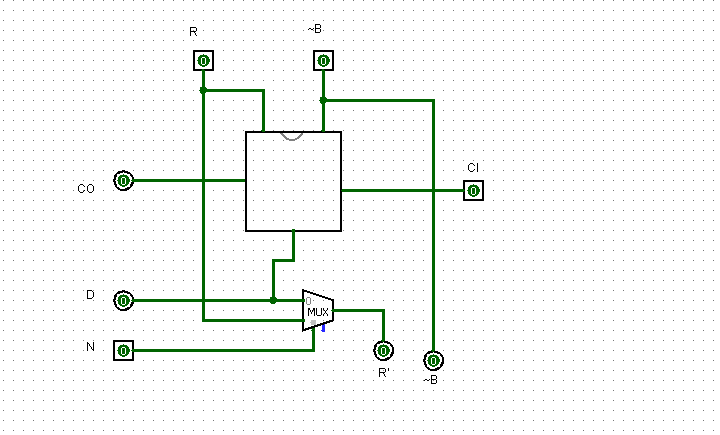
\includegraphics[width=0.6\textwidth]{Divisor_Estagio_Intermediario.png}
		\caption{Circuito Intermediário de um Divisor Completo}
		\label{fig:exemplo}
	\end{figure}

	Detalhes Técnico do Divisor
	
	Tudo se iniciar com a Tabela Verdade de um Somador Completo. Não iremos demonstar o Somador Completo aqui pois o mesmo será discutido em detalhes nesse documento.
	
    A partir do Somador Completo, é feito o encapsulamento em um Circuito integrado que podemos chamar de Bloco central  A partir dai, adicionamos ao bloco um MUX.

 
    Entradas/Saídas marcadas como:

        R (Resto ou A no algoritmo de divisão)

        ~B (Negativo do divisor B,  para subtração)

        CO, CI (carry-out e carry-in)

        D, N ( bits de controle )

        R' (novo valor de R após operação)

 
 Função do Circuito

    Divisor binário sequencial, mais especificamente o bloco que executa a subtração do divisor do valor parcial do dividendo (resto) durante a iteração do algoritmo de divisão restauradora.
 Funcionamento  

    Entradas:

        R → Resto atual (parcial)

        ~B → Inverso de B (para subtração com complemento de dois)

        D, N → Podem ser sinais de controle para o MUX

        CI → Carry-in,   '1' para iniciar subtração com complemento de dois

    Bloco central (Somador):

        Subtrai B de R usando o complemento de dois (R + (~B + 1)), utilizando ~B e CI = 1

    MUX:

        Decide se o resultado da subtração deve ser aceito (se não deu negativo) ou se R deve ser restaurado (no caso do resultado negativo)

        Se a subtração deu negativa, desfazemos (restauramos) e colocamos 0 no quociente.

    Saída:

        R' → Novo valor do resto (pode ser o resultado da subtração ou valor restaurado)

 Resumo

Esse circuito é o estágio intermediário de verificação/restauração usado para a construção do nosso Visivor de 4 Bits.
    Ele realiza R = R - B usando complemento de dois.

    Usa o MUX para restaurar ou manter o valor dependendo do sinal do resultado.

    Produz um novo valor R' para a próxima iteração.



 1.1 \textbf{Divisor} \textbf{Comleto}

   O encapsulamento do bloco intermediário e a conexão com outros blocos, resulta em uma rede de Blocos intermediários capaz de realizar o processo de divisão.

   O divisor feito nesse trabalho é capaz de realizar divisão e apresentar o resto da divisão. Por exemplo, se dividirmos 14 por 3, o resultado será 4 e terá resto 2.
    Para simplificar o circuito de saída, iremos realizar epanas operações cujo resto é zero.

	\begin{figure}[H]
		\centering
		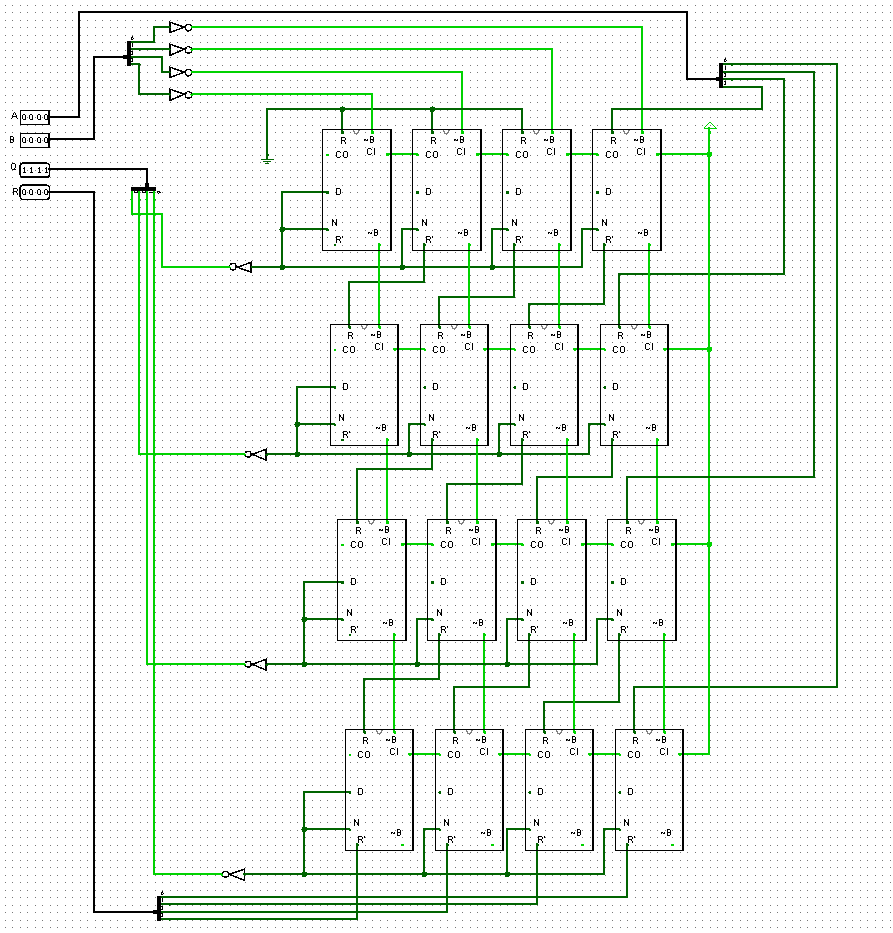
\includegraphics[width=0.6\textwidth]{Divisor_Completo_Final.png}
		\caption{Junção dos blocos para formação do Divisor de 4 Bits}
		\label{fig:exemplo}
	\end{figure}
    
	\chapter{Resultados e Discussão}
	
Abaixo temos a visão geral de nossa ALU	
	\begin{figure}[H]
		\centering
		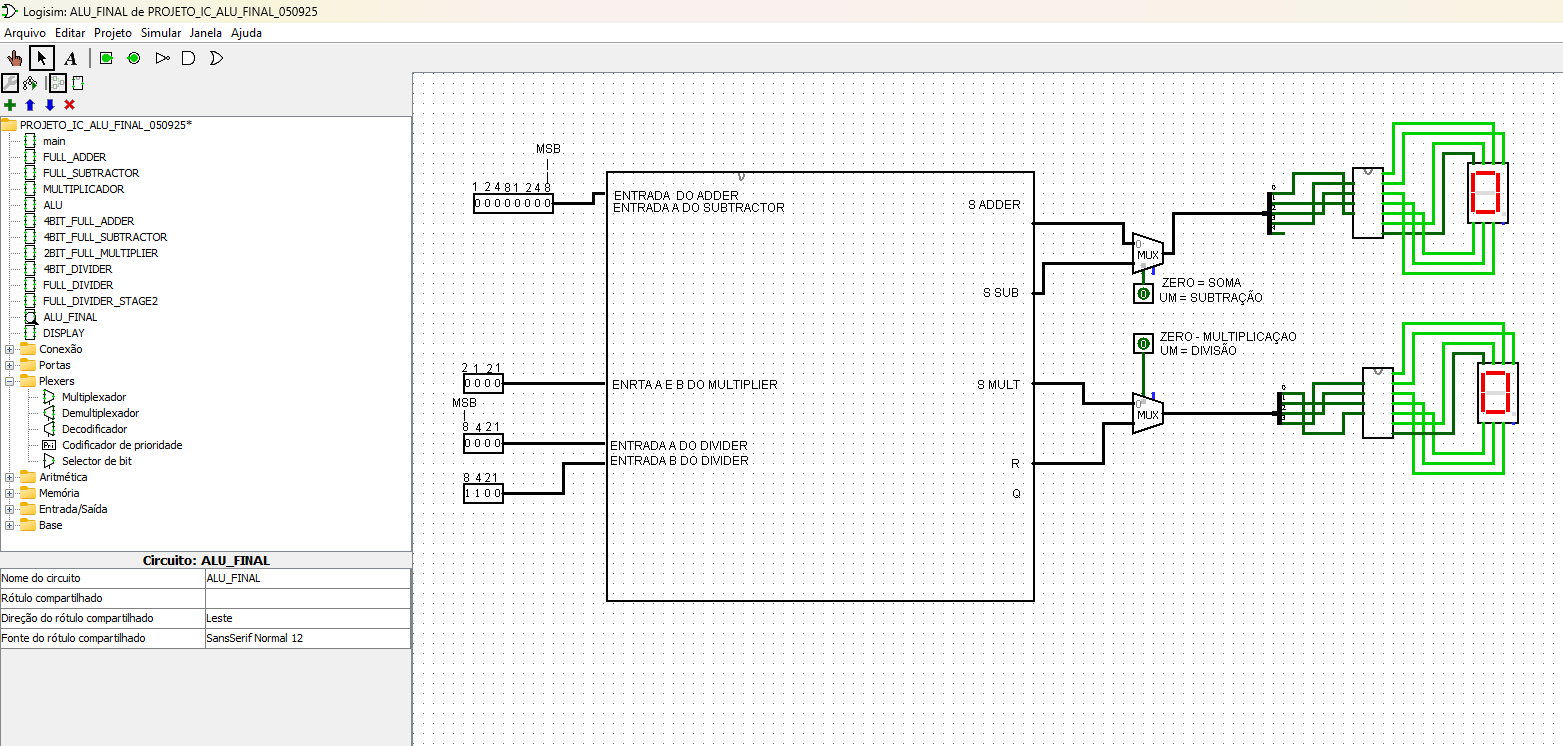
\includegraphics[width=0.6\textwidth]{ALU_Visao_Geral.png}
		\caption{Exemplo de imagem inserida no corpo do trabalho}
		\label{fig:exemplo}
	\end{figure}
	
	Como pode ser observado na Figura~\ref{fig:exemplo}, os resultados são representativos.
	
	\chapter{Conclusão}
	
    Esse trabalho nos possibilitou conhecer como funciona um sistema computacional iniciando pela sua unidade mais básica que é uma porta Lógica.  Ainda que a ALU construida seja capaz de realizar apenas as 4 operações aritiméticas básicas, agora sabemos que a evolução desses circuitos resultam nos atuais sistemas de alta complexidades capazes de executar qualquer tipo de atividade computacional.
    
	
	% Bibliografia
	\cleardoublepage
	\bibliographystyle{abntex2-alf}
	\bibliography{referencias}
	
\end{document}
